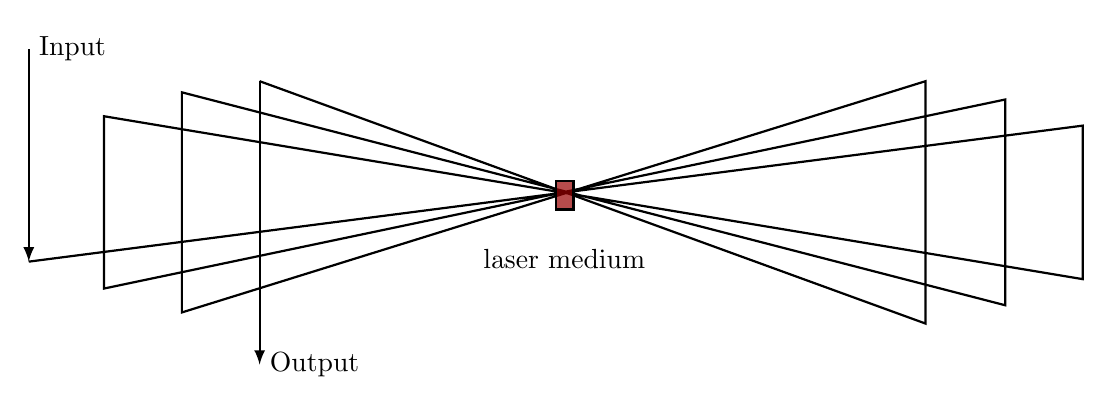
\begin{tikzpicture}[scale=0.9]
    % \draw[step=1cm, gray, very thin] (-5,-5) grid (5,5);
    \draw[thick] (160:5)coordinate(M1) -- 
    (-20:5)coordinate(M2) -- (20:5)coordinate(M3) -- (195:6)coordinate(M4) -- (165:6)coordinate(M5) -- (-14:6)coordinate(M6) -- (14:6)coordinate(M7) -- (190:7)coordinate(M8) -- (170:7)coordinate(M9) -- (-8.9:7)coordinate(M10) -- (8.9:7)coordinate(M11) -- (186:8)coordinate(M12);
    
    \draw[thick, {-latex}] (M1) -- +(0,-4)node[right]{Output};
    \draw[thick, {latex-}] (M12) -- +(0,3)node[right]{Input};
    
    \mirror[angle=125] at (M1);
    \mirror[angle=125-180] at (M2);
    \mirror[angle=55] at (M3);
    \mirror[angle=55+180] at (M4);
    \mirror[angle=125] at (M5);
    \mirror[angle=125-180] at (M6);
    \mirror[angle=55] at (M7);
    \mirror[angle=55+180] at (M8);
    \mirror[angle=125] at (M9);
    \mirror[angle=125-180] at (M10);
    \mirror[angle=55] at (M11);
    \mirror[angle=55+180] at (M12);
    
    \filldraw[fill=red!60!black, fill opacity=0.7, draw=black, thick] (-.52,-.1) rectangle ++(.25,.4);
    \node at (-0.4,-0.8){laser medium};
\end{tikzpicture}